\begin{figure}[!ht]
    \centering
    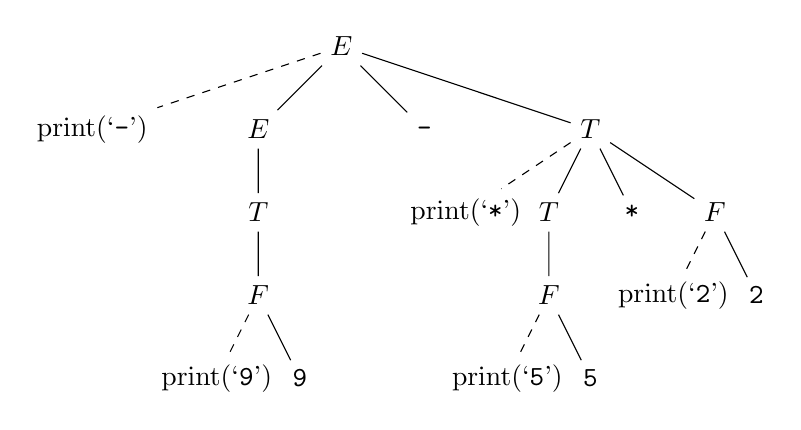
\begin{tikzpicture}
        [
            level distance = 3em, 
            level 1/.style={sibling distance=6em},
            level 2/.style={sibling distance=3em},
        ]
        \node {$E$}
        child {
            node {print(`\texttt{-}')} edge from parent[dashed]
        }
        child {
            node {$E$}
            child {
                node {$T$}
                    child {
                    node {$F$}
                    child {
                        node {print(`\texttt{9}')} edge from parent[dashed]
                    }
                    child {node{\texttt{9}}}
                }
            }
        }
        child {node {\texttt{-}}}
        child {
            node {$T$}
            child {
                node {print(`\texttt{*}')} edge from parent[dashed]
            }
            child {
                node {$T$}
                child {
                    node {$F$}
                    child {node {print(`\texttt{5}')} edge from parent[dashed]}
                    child {node {\texttt{5}}}
                }
            }
            child {node {\texttt{*}}}
            child {
                node {$F$}
                child {node {print(`\texttt{2}')} edge from parent[dashed]}
                child {node {\texttt{2}}}
            }
        }
        ;
    \end{tikzpicture}
    \caption{Parse tree for the input \texttt{9-5*2} for \cref{ex:020301}.}
    \label{fig:020301b}
\end{figure}